\documentclass{article}

\usepackage{a4wide}
\usepackage{amsmath}
\usepackage{amssymb}
\usepackage{graphicx}
\usepackage{hyperref}

\begin{document}

\title{Backpropagation}
\author{Valentin Lhermitte}
\date{\today}

\maketitle

\section{Assigment 1}

The first assigment was to implement all messages for the classes : \texttt{LinearLayer}, \texttt{ReLULayer}, \texttt{SoftMaxLayer} and \texttt{LossCrossEntropy}. 
We also had to implement the gradient method in the \texttt{MLP} class, which compute the gradient of the loss with respect to the parameters of the network. 

Once those implementations done, we train the network on the \texttt{experimental spiral} dataset.
We are going to train the network with 3 different learning rates : 0.2, 1 and 5.
As we can see in the figure \ref{fig:spiral}, the network with a learning rate of 0.2 produce an accuracy of 86\% on the test set.
A learning rate of 1 produce an accuracy of 98.3\% and finally a learning rate of 5 produce an accuracy of 33.3\%.

\begin{itemize}
    \item \textbf{Learning rate of 0.2} : The learning rate is too small, the network would need more epochs to converge to a higher accuracy.
    \item \textbf{Learning rate of 1} : The learning rate is good, the network converge quickly to a high accuracy.
    \item \textbf{Learning rate of 5} : The learning rate is too big, the network diverge and the accuracy is very low.
\end{itemize}

The learning rate is a hyperparameter of the network, it is not learned during the training. It is usually set before training by the user and is usually between 0.001 and 1.

\begin{figure}[h]
    \centering
    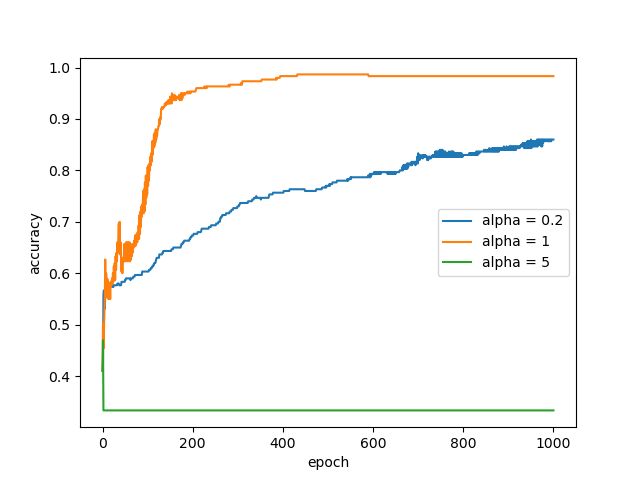
\includegraphics[width=0.6\textwidth]{images/Figure_4.png}
    \caption{Result of the training on the spiral dataset.}
    \label{fig:spiral}
\end{figure}


\section{Assigment 2}

In this assigment, we had to implement the forward and backward message for the compound layer composed of 
the \texttt{softmax layer} and the \texttt{multinominal cross entropy loss}.

Softmax : $ p_k(s) = \frac{e^{s_k}}{\sum_{c=1}^K e^{s_c}} $

Loss : $ l = - \sum_{k=1}^K t_k \log(p_k(x)) $ \\

% Give forward and backward messages for a compound layer composed of the softmax layer:

Forward : 
\begin{align*}
    l &= - \sum_{k=1}^K t_k \log(p_k(x)) \\
      &= - \sum_{k=1}^K t_k \log(\frac{e^{s_k}}{\sum_{c=1}^K e^{s_c}}) \\
      &= - \sum_{k=1}^K t_k (\log(e^{s_k}) - \log(\sum_{c=1}^K e^{s_c})) \\
      &= - \sum_{k=1}^K t_k (s_k - \log(\sum_{c=1}^K e^{s_c})) \\
\end{align*}

Backward :
% \begin{align*}
%     \frac{\partial l}{\partial s_k} &= - t_k + \frac{1}{\sum_{c=1}^K e^{s_c}} \frac{\partial}{\partial s_k} \sum_{c=1}^K e^{s_c} \\
%     &= - t_k + \frac{e^{s_k}}{\sum_{c=1}^K e^{s_c}}  \\
%     &= - t_k + p_k(x) \\
%     &= p_k(x) - t_k
% \end{align*}

% \begin{align*}
%     \frac{\partial p_k(s)}{\partial s_k} &= \frac{\partial}{\partial s_k} \frac{e^{s_k}}{\sum_{c=1}^K e^{s_c}} \\
%     &= \frac{e^{s_k} \sum_{c=1}^K e^{s_c} - e^{s_k} e^{s_k}}{(\sum_{c=1}^K e^{s_c})^2} \\
%     &= \frac{e^{s_k}}{\sum_{c=1}^K e^{s_c}} \frac{\sum_{c=1}^K e^{s_c} - e^{s_k}}{\sum_{c=1}^K e^{s_c}} \\
% \end{align*}


\begin{align*}
    \frac{\partial l}{\partial p_k} &= \frac{-t_k}{p_k} \\ \\
    \frac{\partial p_k}{\partial s_j} &= p_k(\delta_kj - p_j) \\ \\
    \frac{\partial l_k}{\partial s_k} &= \sum_{j=1}^{K} \frac{\partial l}{\partial p_j} \frac{\partial p_j}{\partial s_k} \\
                                      &= p_k - t_k \\
\end{align*}


Show that softmax is invariant to shift in inputs, i.e., $p_k(s') = p_k(s)$ where $s'_k = s_k + c$ for $k \in \{1,...,K\}$ and $c \in \mathbb{R}$.
\begin{align*}
    s'_k &= s_k + c \\
    p_k(s') &= \frac{e^{s'_k}}{\sum_{c=1}^K e^{s'_c}} \\
            &= \frac{e^{s_k + c}}{\sum_{c=1}^K e^{s_c + c}} \\
            &= \frac{e^{s_k} e^c}{\sum_{c=1}^K e^{s_c} e^c} \\
            &= \frac{e^{s_k}}{\sum_{c=1}^K e^{s_c}} \\
            &= p_k(s)
\end{align*}


\section{Assigment 3}

For this assigment, we solve the numeric instability by taking into account the remark made in the assigment 2.
We also had to introduce the softmax inside of the cross entropy loss. 
The computation for the delta isn't a division anymore but now a substraction. This allow us to avoid numerical instability. 

The accuraccy of this classifier is now 99\% and a loss of 0.02 for a 100 epochs (see fig \ref{fig:MNIST}).

\begin{figure}[h]
    \centering
    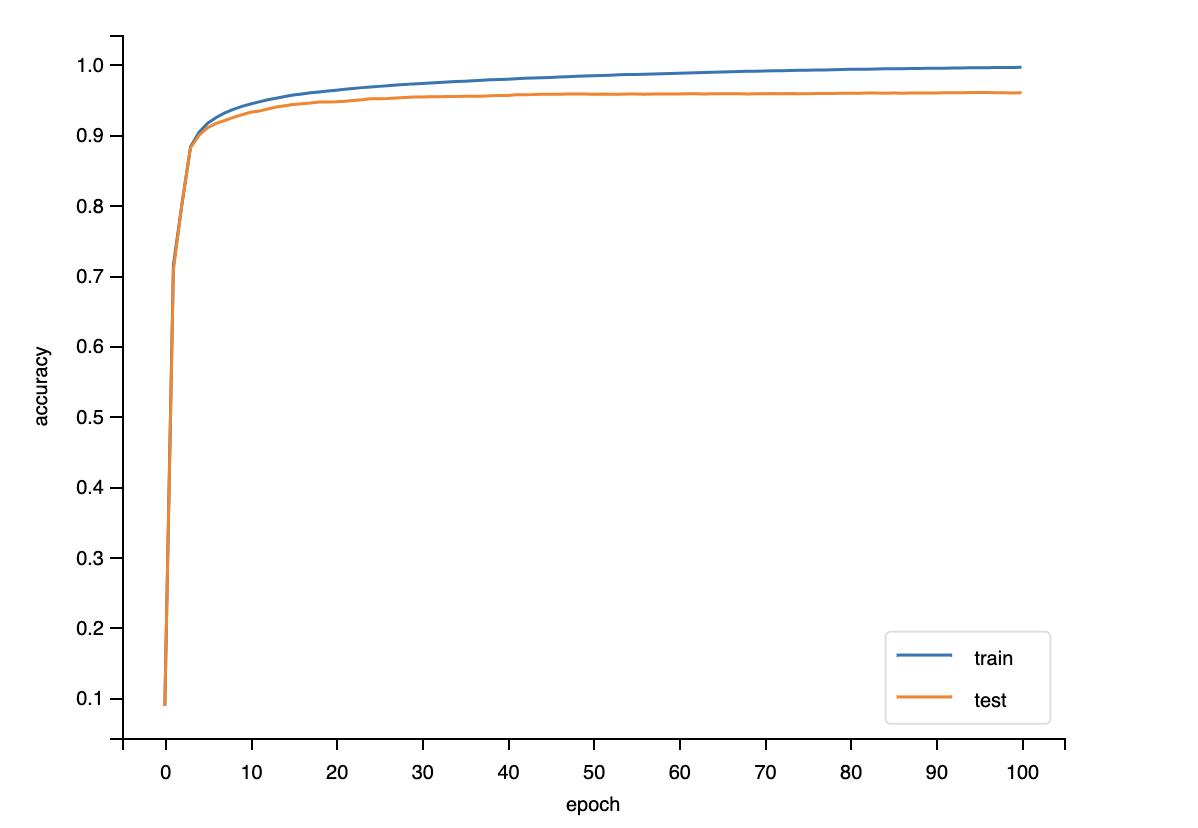
\includegraphics[width=0.7\textwidth]{images/Figure_5.png}
    \caption{Result of the training on the MNIST dataset.}
    \label{fig:MNIST}
\end{figure} 
\end{document}